\chapter{Analýza požiadaviek na systém}\label{anal}
Na vytvorenie návrhu z~kapitoly \ref{navrh} je najskôr potrebné analyzovať používateľov, ich požiadvky~a~potreby na systém vykurovania. 
Postup a konkrétna analýza používateľov je~v~podkapitole \ref{analyza-user}. 
Existujúce riešenia z~podkapitoly \ref{analyza-solutions} poskytujú informácie o~riešeniach tejto problematiky. 
Tie poskytujú možnosti inšpirovať, poučiť sa z~daných riešení pri návrhu a~zároveň je možné ich využiť v~implementácii. 
Pri návrhu je veľmi dôležité zohľadniť a~dosiahnuť požiadavky zadané firmou Logimic, ktoré sú analyzované v~podkapitole \ref{Logimic}. 
Na~základe získaných informácii z~tejto kapitoly je v~podkapitole \ref{analyza-requirements} vytvorený výstup a~záver analýzy.

\section{Analýza používateľov}\label{analyza-user}
Používateľov som si rozdelil do dvoch skupín podľa toho, v~akých priestoroch by mohol byť systém implementovaný. 
To na používateľov v~domácnosti obsiahnutých v~podsekcii \ref{analyza-user-home} a~vo~firemných priestoroch v~podsekcii \ref{analyza-user-bussiness}. 
Toto rozdelenie bolo vytvorené a zvolené z~dôvodu rozličných požiadaviek na systém ovládania. 
Výstup analýzy je tak isto rozdelený do~dvoch časti, pretože požiadavky pre ovládanie vo firemných priestoroch sú rozdielne. Výsledky vychádzajú z~predošlých prieskumov. 
Firemné požiadavky boli diskutované s~kontateľom firmy \emph{Virtuálny správca budov, s.r.o.}\footnote{Dostupnej na stránke: \url{https://vsb-po.sk}.}, s~pánom Ing.~Slavomírom Satvárom.

\subsection*{Postup analýzy}
Informácie od potencionálnych používateľov som sa rozhodol získavať prostredníctvom interaktívneho dotazníka\footnote{Dostupný na stránke: \url{https://forms.gle/2kGT15zaL6VF1hxS7}. 
Dáta z~dotazníka prebrané dňa 23.03.2013.}, vytvoreného na platforme \emph{Google forms}. 
Recipientom tohto formulára boli rodinný príslušníci, rovesníci a spolužiaci. 
Formulár obsahuje sadu otázok zameraných na interakciu používateľov so systémom, očakávané funkcie systému a všeobecne identifikáciu požiadaviek na systém.

\subsection{Výstup analýzy v~domácnosti}\label{analyza-user-home}
V~domácnosti je používateľom väčšinou jednotlivec, ktorý chce hlavne ušetriť na vykurovaní alebo prípadne ho chce automatizovať. 
Priemerný používatelia bývajú v~bytoch alebo bytových domoch a majú v~domácnosti nainštalované radiátorové kúrenie. Tieto byty sú väčšinou trojizbové. 
V~každej izbe sa nachádza priemerne jeden radiátor. 
Medzi požiadavky rezidentov patrí manuálne a diaľkové ovládanie kúrenia, detekcia otvoreného okna, nastavovanie vykurovacích rozvrhov, grafický prehľad spotreby, grafický prehľad teploty miestností a prehľad výkonu radiátora. 
Ďalšie požiadavky sú, aby inštalácia bola čo najjednoduchšia a očakávajú jednoduchú a prehľadnú aplikáciu na ovládanie vykurovania. 

\subsection{Výstup analýzy vo firemných priestoroch}\label{analyza-user-bussiness}
Vo firemných priestoroch je zákazníkom práve firma, ktorá chce hlavne ušetriť na vykurovaní alebo ho prípadne chce automatizovať.
Väčšie firmy majú často väčší počet budov s~väčším počtom poschodí.
Preto mimo už spomínané funkcie pre jednotlivé byty, vyžadujú komplexnejšie delenie a priraďovanie zariadení do miestností, miestnosti do poschodí a poschodia do budov. 
Ďalšou požiadavkou bolo vypnutie alebo zapnutie kúrenia podľa rozvrhu a rezervácie miestností, teda v~prípade, že zamestnanec si rezervuje miestnosť alebo ak sa bude v~danej miestnosti čoskoro konať stretnutie, daná miestnosť sa dopredu vyhreje.
K~manuálnemu ovládaniu bola požiadavka aby zamestnanci boli schopný len dočasne zmeniť cieľovú teplotu radiátora. 

Tento systém by mohol byť využiteľný aj správcami budov, ktorým by mohol priniesť lepšiu kontrolu a prehľad o~využití tepla v~budovách. K~tomu by ale potrebovali novú radu funkcií. Hlavne rozsiahlych štatistických prehľadov, výpočtov spotrebovaného tepla a~iných. Zameranie systému týmto smerom je zvýhodňované slovenskou legislatívou, kde od~roku 2027 pravdepodobne príde do platnosti zákon o~elektronickom zbere dát\footnote{Predbežné stanovisko dostupné na \url{https://www.google.com/url?sa=t&rct=j&q=&esrc=s&source=web&cd=&cad=rja&uact=8&ved=2ahUKEwjAteX2-eL-AhXhgP0HHZs1ArIQFnoECAsQAQ&url=https\%3A\%2F\%2Fwww.nrsr.sk\%2Fssez\%2FdownloadDoc.ashx\%3FDocID\%3D5099&usg=AOvVaw097BQtvskILLjOxhEVcfjT}}.

\section{Existujúce riešenia}\label{analyza-solutions}
Riešením inteligentného vykurovania sa už zaoberal väčší počet firiem a vďaka tomu vzniklo aj väčšie množstvo riešení tejto problematiky. 
V~tejto podkapitole je niekoľko týchto riešení analyzovaných na základe informácii dostupných od predajcov, a sú z~nich vyvodené ich plusy, mínusy a spôsob riešenia tejto problematiky. 
Ďalej sú rozdelené podľa technológie, ktorú využívajú na bezdrôtové prepojenie zariadení.

\subsection*{IQRF}
Komerčné riešenie využívajúce túto technológiu je len jedno od Slovenskej firmy \emph{Austyn}\footnote{Stránka predajcu \url{https://austyn.sk}.}. 
Výhodou tejto technológie je pripojenie zariadení metódou každý s~každým, teda technológiou \emph{mesh networking} za použitia proprietárneho IQMESH. 
Táto kombinácia vytvára značnú výhodu v~prenose dát pri väčšom počte zariadení na väčšom priestore. 
Problémom je ale nutnosť zapojenia so do \emph{IQRF Alliance} pre možnosť využitia ich riešení.
Konkrétne riešenie je možné vďaka inteligentnej hlavici od firmy \emph{Austyn}, ktorá je pripojená do siete IQRF. 
S~využitím IQRF brány je možné potom ovládať danú hlavicu vzdialenou aplikáciou. Informácie o~hlavici sú zo zdroja~\cite{Austyn_hlavica}. 
Výhodou tejto hlavice\footnote{Dostupná z~\url{https://www.iqrfalliance.org/marketplace/mag-ra}.}, ktorú môžete vidieť na~obrázku \ref{fig:IQRF-TRV}, je jednoduchá a rýchla inštalácia aj vďaka automatickej adaptácii na ventil. 
Autonómny ovládač zabudovaný priamo v~hlavici pre jej nezávislosť od internetového pripojenia. 
Možnosť alternatívneho, priamo pripojeného merania teploty vyvedeným káblom. 
Voliteľne môže byť výhodou dodatočná zabezpečovacia konštrukcia. 
Celé riešenie s~využitím aplikácie potom získava funkcie ako automatická regulácia kúrenia, možnosť nastaviť týždenný program, meranie teploty, stav ventilu, stav hlavice a jej bateriek a detekcia otvoreného okna.
K~tomu podporuje nemrznúcu a koróznu ochranu a možnosť ovládať hlavicu aj manuálne. Veľkým problémom tohto riešenia je, že nie je otvorené a je integrované firmou \emph{Austyn} ako kompletné riešenie. 
Pre možnosť využitia tohto riešenia by boli potrebné dlhších komunikácie a dohôd s~firmou \emph{Austyn}.
\begin{figure}[H]
    \centering
    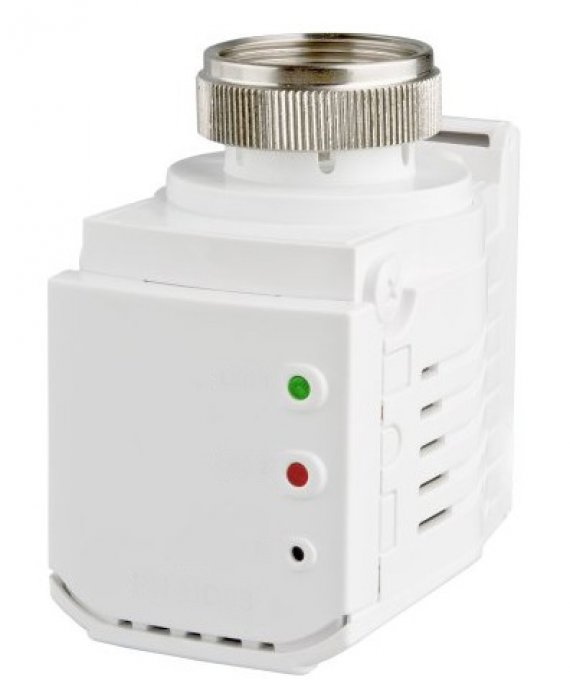
\includegraphics[scale=0.4]{obrazky-figures/m_retusovana-hlavica.jpg}
    \caption{Inteligentná hlavica MAG RA od firmy \emph{Austyn}.}
    \label{fig:IQRF-TRV}
\end{figure}


Možné riešenie s~technológiou IQRF je vyskladať samostatne hlavicu ovládateľnú elektronicky a pripojiť k~nej \emph{IQRF modul}\footnote{Napríklad modul dostupný z~\url{https://eshop.iqrf.org/cz/bezdratove-moduly-tr}.}, ktorý by slúžil ako prijímač a vysielač. 
Ten by ďalej komunikoval s~\emph{IQRF bránou}\footnote{Napríklad brána dostupná z~\url{https://eshop.iqrf.org/cz/pristupove-brany}.}.  
\subsection*{LoRaWAN}
Túto technológiu využívajú dvaja výrobcovia v~dvoch konkrétnych riešeniach. Prvou je Nemecká firma \emph{Micropelt}\footnote{Stránka výrobcu \url{https://www.micropelt.com/en/}.}. 
Vyvinuli inteligentnú hlavicu\footnote{Dostupnú z~\url{https://www.smartbuildingproducts.co.uk/product/micropelt-mlr003-lorawan-actuator}.}, ktorú môžete vidieť na obrázku \ref{fig:LORA-MICROPELT}. 
Informácie o~tejto hlavici sú zo zdroja \cite{Micropelt_hlavica}. Výhodou tejto hlavice je vysoká úspora energie, nakoľko je energeticky sebestačná. 
Energiu, ktorú využíva získava konverziou teplotných rozdielov horúceho radiátora a okolitého vzduchu na elektrickú energiu. 
Tým sa eliminuje potreba častej výmeny baterií. Hlavica ma robustný dizajn so zameraním na verejné priestory. 
Preto hlavici chýba možnosť manuálneho ovládania. Ovládanie je možné iba rádiovou LoRaWAN technológiou, ktorá je opísaná v~\ref{iot-trasport}. 
Medzi jej funkcie patrí percentuálne otvorenie ventilu alebo nastavenie konkrétnej teploty pomocou teplotného senzoru v~hlavici. 
Hlavica zároveň odosiela údaje o~teplote, stave baterky a motoru a správy o~spotrebe a~generácii energie. 
V~prípade, že je spotreba dlhodobo vyššia ako generácia, je možné hlavicu cez USB port dobiť.
Najdôležitejším prvkom tohto riešenia je, že je otvorené a ponúka dokumentáciu\footnote{Dostupnú z~\url{https://micropelt.atlassian.net/wiki/spaces/MH/pages/2981889/MLR003RiEU61-07+EN}.} obsahujúcu modely a spôsoby komunikácie s~hlavicou. 
To znamená, že~za~použitia ľubovoľnej \emph{LoRaWAN brány} je možné po pripojení priamo ovládať hlavicu už~navrhnutými príkazmi.
Inštalácia tejto hlavice ale môže obnášať komplikácie kvôli kompaktibilite s~ventilom radiátora, nakoľko pasuje iba na závit \emph{M30 x 1,5}. 
Problém môže nastať aj v~prípade častejšej komunikácie s~bránou, kedy je očakávane, že generovanie energie bude nedostatočné.

\begin{figure}[H]
    \centering
    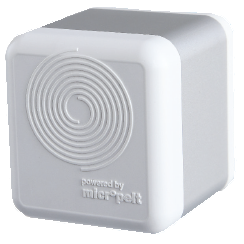
\includegraphics[scale=0.5]{obrazky-figures/_MLR003_UK-CERT_980x385_A_edited.png}
    \caption{Inteligentná hlavica MLR003 od firmy \emph{Micropelt}.}
    \label{fig:LORA-MICROPELT}
\end{figure}

Druhým výrobcom je Bulharská firma \emph{MClimate}\footnote{Stránky výrobcu sú \url{https://mclimate.eu}.}. 
Táto firma vyvinula inteligentnú hlavicu\footnote{Dostupnú z~\url{https://mclimate.eu/products/vicki-lorawan}.}, komunikujúcu technológiou LoRaWAN opísanou v~\ref{iot-trasport}. Obrázok \ref{fig:LORA-MCLIMATE} zobrazuje túto hlavicu.
Informácie o~tejto hlavici sú zo zdroja \cite{vicki}.
Výhodou tejto hlavice je možnosť manuálneho ovládania, čo môže predstavovať výhodu v~prostredí domova. 
Na rozdiel ale od spomínanej MLR003 od firmy \emph{Micropelt} je hlavica \emph{Vicki} plne závislá na batériách. 
Výrobca však sľubuje výdrž zariadenia na jeden set batérii v~období niekoľkých rokov. 
Medzi funkcie hlavice patrí nastavenie požadovanej teploty buď manuálne alebo diaľkovo príkazmi.
Ovládanie a reguláciu pomocou externých senzorov.
Digitálny displej zobrazujúci momentálne nastavenú teplotu. 
Možnosť zamknúť manuálne ovládanie. 
Inštalácia hlavice by nemala byť komplikovaná vďaka kompatibilite so značným počtom ventilov.
Táto hlavica je tak isto ako MLR003 je otvorená a má prístupnú rozsiahlu dokumentáciu\footnote{Dostupnú z~\url{https://docs.mclimate.eu/mclimate-lorawan-devices/devices/mclimate-vicki-lorawan}.}. 
Vďaka tomu je možné ovládanie hlavice z~rôznych aplikácii.
\begin{figure}[H]
    \centering
    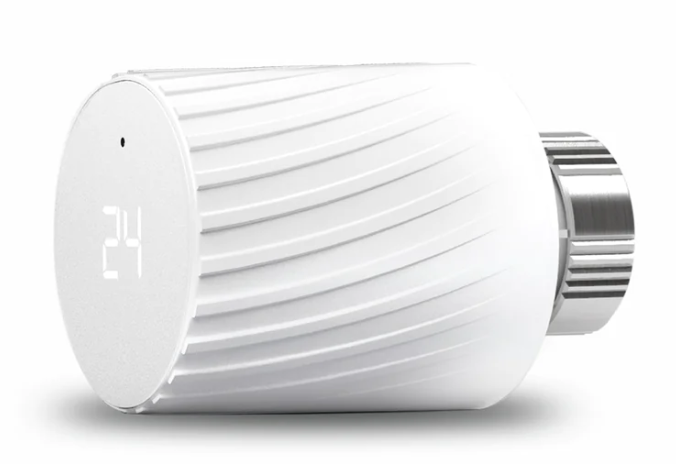
\includegraphics[scale=0.285]{obrazky-figures/vicky.png}
    \caption{Inteligentná hlavica Vicki od firmy \emph{MClimate}.}
    \label{fig:LORA-MCLIMATE}
\end{figure}

\subsection*{ZigBee}
Technológia ZigBee sa pýši najväčšiemu zastúpeniu komerčných riešení. 
Táto technológia je opísaná v~podkapitole \ref{iot-trasport}. 
Výrobcov riešení inteligentného vykurovania je tak isto obrovské množstvo. 
Každý ponúka trošku iné riešenie s~troška inými výhodami a nevýhodami. 
Všetky sa ale zameriavajú na prepojenie s~domácimi asistentmi alebo inými proprietárnymi  aplikáciami.
Výrobcovia teda neponúkajú možnosť využiť ich riešenia a hlavice v~iných aplikáciách ako nimi podporovaných. 
Jedná sa hlavne o~\emph{Google Assistant}, \emph{Amazon Alexa}, \emph{Tuya}, \emph{Apple Siri} alebo konkrétnu mobilnú aplikáciu výrobcu na systéme \emph{Android} alebo \emph{iOS}. 
Obecne všetky takéto hlavice vyžadujú napájanie z~batérii a majú nejakú formu displeja. 
Medzi obecné funkcie patrí vzdialené ovládanie ventilu, nastavenie požadovanej teploty alebo nastavenie plánov a rozvrhov. 
Pri pripojení na domáceho asistenta získavajú radu ďalších možností, ako napríklad spustenie vyhrievania miestnosti ak sa v~nej nachádzate alebo detekcia otvorených okien a tak ďalej. 
Väčšina hlavíc nemá pri inštalácii problém, nakoľko sú väčšinou kompatibilné so všetkými ventilmi alebo výrobcovia k~baleniu pridávajú adaptéry na ventil.
Každé riešenie od konkrétneho výrobcu vyžaduje bránu od tohto istého výrobcu. 
Tým vzniká problém, kde pre ideálne riešenie je potrebné využívať produkty iba od~jedného výrobcu, aby nebolo potrebné mať v~domácnosti zapojených niekoľko brán. 
Tieto spomínané problémy je ale možné obísť napríklad prekladom zo ZigBee komunikácie na napríklad \emph{MQTT}\footnote{Štandartný správový IoT protokol. Viac na stránkach \url{https://mqtt.org}.}, ktorému rozumie takmer každé IoT zariadenie.
Toto ale nie je v~súlade s~podmienkami predajcu a ešte to~je aj zbytočne komplikované.

\section{Logimic}\label{Logimic}
Jedná sa o~firmu\footnote{Dostupná na \url{https://www.logimic.com}.}, ktorá hlavne vytvára software na objednávku so zameraním na IoT aplikácie v~oblasti inteligentných miest spomínaných v~podkapitole \ref{iot-smartcity}.
Klienti firmy pochádzajú z~európskych krajín a Severnej Ameriky. 
Logimic pre nich vytvára rozhrania, pripravuje hardware a všeobecne inak pripravuje riešenie pre požadovaný systém. 
Jednou z~nových oblastí ktorým, by sa firma Logimic chcela venovať je aj systému pre inteligentné vykurovanie.

Na základe konverzácii s~pánom doktorom Michalom Valným a~s~pánom inžinierom Františkom Mikulu, bolo možné určiť požiadavky a očakávané výstupy firmy Logimic. 
Tá~očakáva, aby v~ACADA platforme, aplikácii iTemp bolo možné ovládať a nastavovať systém vykurovania. 
Na to očakáva jednoduché a prehľadné používateľské rozhranie. Aplikáciu iTemp môžete vidieť na obrázku \ref{fig:iTemp}.
Platforma ACADA (skratka z~anglického \emph{Asset Control and Data Acquisition}) integruje koncové zariadenia a aplikácie 3-tích strán, správu aktív, správu pracovných požiadavkou a prepojenia s~obyvateľmi mesta alebo zákazníkmi.

iTemp je bezdrôtové riešenie monitoringu vnútorného a vonkajšieho prostredia najmä teploty a vlhkosti. 
Pracuje s~mnohými typmi senzorov ako je IQAROS sada, LoRa teplotné senzory a ďalšie. 
iTemp je riešenie v~momentálnom neustálom vývoji a firma Logimic zadala požiadavku ho rozšíriť o~ovládanie vykurovania.

\begin{figure}[H]
    \centering
    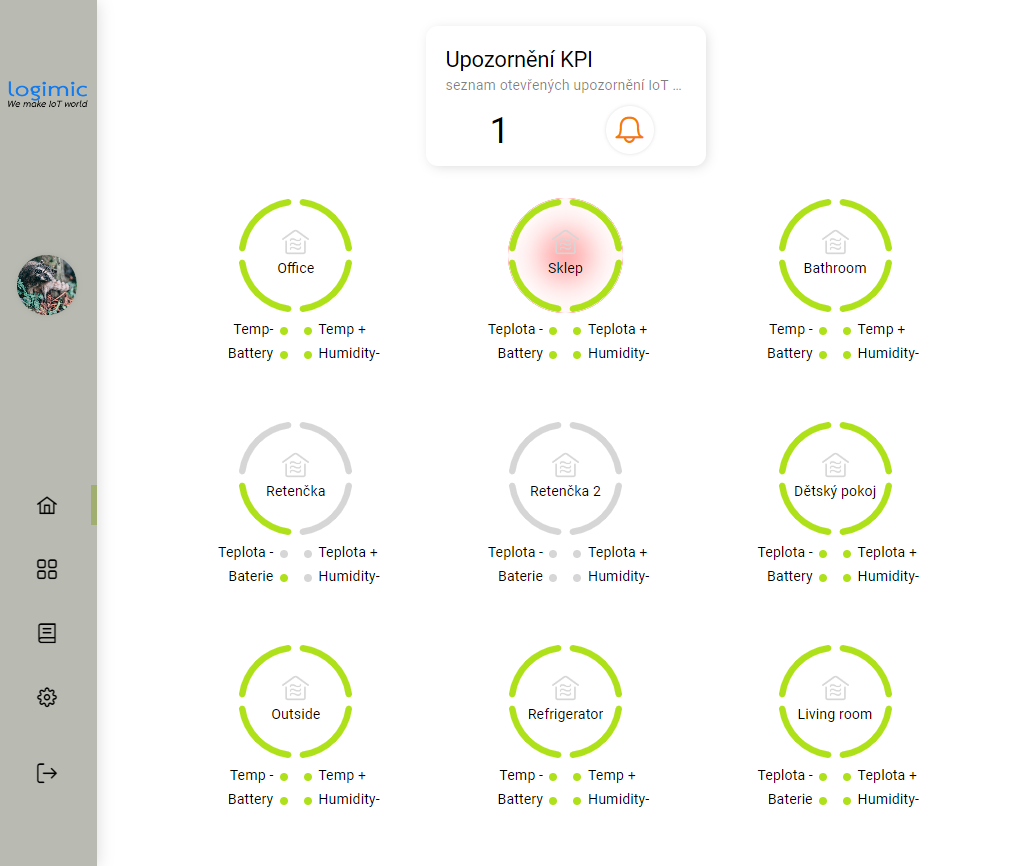
\includegraphics[width=\textwidth]{obrazky-figures/Screenshot_12.png}
    \caption{Domovská obrazovka aplikácie iTemp.}
    \label{fig:iTemp}
\end{figure}

\section{Výsledné požiadavky}\label{analyza-requirements}
Na základe analýzy potencionálnych používateľov z~podkapitoly \ref{analyza-user} a  existujúcich riešení z~podkapitoly \ref{analyza-solutions} a konkretizovaní požiadaviek firmi Logimic z~podkapitoly \ref{Logimic} sú v~tejto podkapitole vyvedené konkrétne požiadavky na systém. 
Požiadavky sú značne skresané za~účelom dosiahnutia časového rozsahu bakalárskej práce.

Zameraním vývoja sa stanú byty, kde výhrevným telesom bude radiátor. 
Ten bude ovládaný regulátorom od firmy \emph{MClimate Vicki}. 
Tým pádom bude využitá technológia \emph{LoRaWAN}. K~tomu bude potreba ďalších teplotných senzorov, tiež využívajúcich technológiu LoRaWAN, aby stačila jedna brána. 
Najdôležitejšie je vytvoriť posielanie a odosielanie dát z~riešenia iTemp na zariadenia. 
Pokračovať by sa malo vo vytvorení obsluhy zariadení a algoritme inteligentného vykurovania.
Funkciami inteligentného kúrenia by malo byť manuálne a diaľkové ovládanie teploty v~miestnosti aj za pomoci externých senzorov, možnosť zamknutia manuálneho ovládania a ovládanie teploty aj v~prípade výpadku internetu.
Používateľské rozhranie by malo vychádzať z~existujúceho riešenia iTemp, rozšíreného o~odosielanie príkazov na zariadenia.